\documentclass[11pt,letterpaper]{article}

\usepackage{latexsym,graphicx}
\usepackage{amsmath,amssymb}
\usepackage{amsthm}
\usepackage{enumerate}
\usepackage{graphicx}
\usepackage{cleveref}
\usepackage{algorithmic}
\usepackage{algorithm}

% Useful macros
\newcommand{\E}[1]{\mathbf{E}\l[#1\r]}
\newcommand{\problem}[1]{\section*{Problem #1}}
\renewcommand{\l}{\left}
\renewcommand{\r}{\right}
\renewcommand{\iff}{\Leftrightarrow~}
\newcommand{\intff}{\int_{-\infty}^\infty }
\newcommand{\intzf}{\int_0^\infty }
\newcommand{\intpp}{\int_{-\pi}^\pi }
\newcommand{\sumzf}[1]{\sum_{#1=0}^\infty}
\newcommand{\sumff}[1]{\sum_{#1=-\infty}^\infty}
\newcommand{\Bin}{\text{Bin}}
\newcommand{\pfrac}[2]{\l(\frac{#1}{#2}\r)}
\renewcommand{\bf}{\textbf}
\newcommand{\zm}[1]{z^{-#1}}
\renewcommand{\P}[1]{\mathbf{P}\l\{#1\r\}}
\newcommand{\Var}[1]{\mathbf{Var}\l(#1\r)}
\newcommand{\Poiss}{\text{Poiss}}
\newcommand{\Geom}{\text{Geom}}
\newcommand{\Skew}{\text{\bf{Skew}}}

\newtheorem{lemma}{Lemma}
\newtheorem{theorem}[lemma]{Theorem}
\newtheorem{informaltheorem}[lemma]{Informal Theorem}
\newtheorem{informallemma}[lemma]{Informal Lemma}
\newtheorem{corollary}[lemma]{Corollary}
\newtheorem{definition}[lemma]{Definition}
\newtheorem{proposition}[lemma]{Proposition}
\newtheorem{question}{Question}
\newtheorem{example}[lemma]{Example}
\newtheorem{remark}[lemma]{Remark}
\newtheorem{claim}{Claim}
\newtheorem{fact}{Fact}
\newtheorem{challenge}{Challenge}
\newtheorem{observation}{Observation}
\newtheorem{openproblem}{Open Problem}
\newtheorem{openquestion}{Open question}
\newcommand{\todo}[1]{\noindent \colorbox{green}{\begin{minipage}{\linewidth}{\bf TODO:} #1\end{minipage}}}

\newcommand{\beq}{\begin{equation}}
\newcommand{\eeq}{\end{equation}}
\newcommand{\beas}{\begin{eqnarray*}}
\newcommand{\eeas}{\end{eqnarray*}}

\newcommand{\poly}{\mathrm{poly}}
\newcommand{\eps}{\epsilon}
\newcommand{\e}{\epsilon}
\newcommand{\polylog}{\mathrm{polylog}}
\newcommand{\rob}[1]{\left( #1 \right)} %Round Brackets
\newcommand{\sqb}[1]{\left[ #1 \right]} %square Brackets
\newcommand{\cub}[1]{\left\{ #1 \right\} } %curly brackets
\newcommand{\rb}[1]{\left( #1 \right)} %Round
\newcommand{\abs}[1]{\left| #1 \right|} %| |
\newcommand{\zo}{\{0, 1\}}
\newcommand{\zonzo}{\zo^n \to \zo}
\newcommand{\zokzo}{\zo^k \to \zo}
\newcommand{\zot}{\{0,1,2\}}
\newcommand{\norm}[1]{\left\lVert#1\right\rVert}
%
%\newcommand{\en}[1]{\marginpar{\textbf{#1}}}
%\newcommand{\efn}[1]{\footnote{\textbf{#1}}}
\newcommand{\bR}{\mathbb{R}}
\newcommand{\bE}{\mathbb{E}}

%%%%%%%%%%%%%%%%%%%%%%%%%%%%%%%%%%%%%%%%%%%%%%%%%%%%%%%%%%%%%%%%

\begin{document}



\section{Knowledge Modeling - Graph Databases}
The goal is to turn schema-less data into data with schema by exploiting the embedded schema information and identifying the structural regularities in a given database. 

\subsection{Graph Data Model}
The graph data model is used as it can generalize common data models (e.g. relational, XML, RDF, etc).
\subsubsection{Formal Definition} 
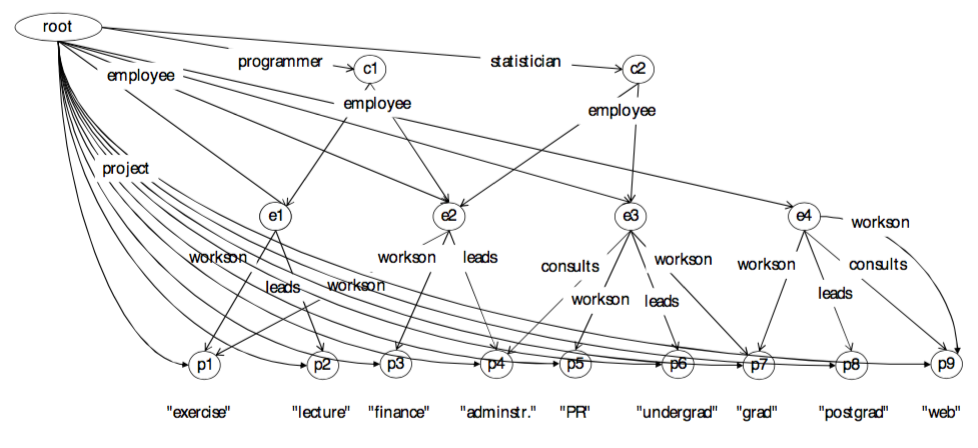
\includegraphics[width=\textwidth]{figures/data_graph.png}
\begin{itemize}
  \item Data graph: D = (V, E, R) is a labeled, rooted and directed graph. 
  \item V is a set of nodes
  \item E $\subseteq$ V x L x V is a set of labeled edges, they determine the meaning of the data values stored in the leaves
  \item R $\subseteq$ V is a set of root nodes that have no incoming edges. All nodes in V are reachable from some root in R
  \item A $\subseteq$ V are the atomic nodes = set of leaf nodes storing typed data values
  \item C $\subseteq$ A x U x T is the data stored in D, where U is the domain of all data values and T are the data types
\end{itemize}

\subsubsection{Structural Properties}
We can enumerate the paths starting from the root to capture the structure of the data graph. A possible schema would be to use a trie enumerating those paths and labeling the leaf nodes with the data type that is found in the graph database. However, it contains many redundant structures so it would be better to combine different subgraphs into a common graph structure. 

\subsubsection{Simulation and Schema Graphs}
Simulation is used to provide a criterion to decide whether a schema graph S correctly captures the structure of a data graph D. A schema graph may use alternate labels or wildcards on edges. Condition: for every node d in D reached by a path p starting from the root there exists a corresponding node s in S reachable by the same path and the types of the leaf nodes are the same in case d is a leaf node. S simulates D is denoted as D $<$ S.

More formal definition of the simulation relationship among labelled graphs:
\begin{itemize}
  \item Given graphs G$_{1}$, G$_{2}$ and relation R $\subseteq$ V$_{1}$ x V$_{2}$, then R is a simulation if for all labels l $\in$ L and for all x$_{1}$, y$_{1}$ $\in$ V$_{1}$ and for all x$_{2}$ $\in$ V$_{2}$ it holds that if x$_{1}$ $\rightarrow$$_{l}$ y$_{1}$ and R(x$_{1}$, x$_{2}$) then there exists y$_{2}$ $\in$ V$_{2}$ such that R(y$_{1}$, y$_{2}$) and x$_{2}$ $\rightarrow$$_{l}$ y$_{2}$
  \item If it holds, G$_{2}$ simulates G$_{1}$ and we can write G$_{1}$ $<$ G$_{2}$
\end{itemize}

We have to extend the concept of simulation relationship for the graph data model:
\begin{itemize}
  \item A schema graph S is a schema for a data graph D if there exists a rooted, typed simulation of D using S (that may contain wildcards and alternate labels). We require that root and leaf nodes in the data graph are related to root and leaf nodes in the schema graph. 
  \item Rooted simulation: R(r$_{1}$, r$_{2}$) for the roots r$_{1}$ and r$_{2}$  
  \item Typed simulation: for all x, y if R(x, y) and y is an atomic type then x must be an atomic node with content of that type
  \item For wildcards and alternate labels the label in the data graph has to be contained in the set of labels specified by these extended schema edge labels: if x$_{1}$ $\rightarrow$$_{l}$ y$_{1}$ then x$_{2}$ $\rightarrow$$_{l}$ y$_{2}$ or x$_{2}$ $\rightarrow$ $_{\_}$ y$_{2}$ or x$_{2}$ $\rightarrow$$_{l|k|...}$ y$_{2}$

\end{itemize}

\subsubsection{Classification by Schema Graphs}
We can define the rooted simulation R as a table with S nodes on the left (Class) and corresponding nodes in D on the right (Instances). The database schema classifies the data in the database.

\paragraph{Multiple classification}: a data node may belong to multiple classes. Two different valid simulations could classify the same data node in different classes (as it requires to be classified in at least one class, but not all possible classes), which could lead to ambiguous classification.

\paragraph{Maximal simulations}: it guarantees that the resulting classification is unique. Given two simulations R$_{1}$ and R$_{2}$ between a data graph and a schema graph the following holds: D $<$$_{R1}$ S and D $<$$_{R2}$ S then  D $<$$_{R1 \cup R2}$ S. The maximal simulation can be computed as a fixpoint iteration. 

\paragraph{Fixpoint iteration}: We start from the total relation between all nodes of D and S, i.e., data instances belong to all classes. Then we stepwise eliminate those pairs in R that violate the simulation condition. That is, whenever a pair should be contained in R we check whether a corresponding link exists in the data graph.
\begin{algorithm}
\caption{Fixpoint iteration for data graph D, schema graph S}
\begin{algorithmic} 
\STATE $R' \leftarrow \emptyset$
\STATE $R \leftarrow \{ (o, c) | o \in D, c \in S \}$
\WHILE{$R \neq R'$}
\STATE $R' \leftarrow R$
\STATE $R \leftarrow  \{ (o, c) |$ all $(o, c)$ such that either o is atomic value and c its type or there exists $(o', c') \in R'$ and $o \rightarrow _{l} o' \in D$ and $c \rightarrow _{l} c' \in S \}$
\ENDWHILE
\end{algorithmic}
\end{algorithm}

\subsubsection{Refining Schemas}
\begin{itemize}
\item Refinement is needed when a schema evolves and becomes more precise over time as more information on the databases become available. 
\item We say that schema S$_{1}$ subsumes schema S$_{2}$ if S$_{1}$ contains less detail and is more general than schema S$_{2}$. It implies that all databases that conform to S$_{2}$ also conform to S$_{1}$
\item This is the case if S$_{2}$ $<$ S$_{1}$. So if S$_{2}$ is a schema for D (D $<$ S$_{2}$) then we can conclude that D $<$ S$_{1}$ and therefore S$_{1}$ is also a schema for D.
\end{itemize}

\subsection{Schema Extraction}
The goal is to automatically construct a schema graph from the data graph. It should be:
\begin{itemize}
\item \textbf{Accurate}: every path that occurs in the schema graph occurs in the data graph and vice versa
\item \textbf{Concise}: every path occurs only once
\end{itemize}
It is called a \textbf{data guide}. Data guide nodes correspond to subsets of data graph nodes. Its root node is the set containing the data graph root. 
\subsubsection{Data Guide Construction}
For each data guide node constructed and for each edge label of an  edge leaving in the data graph some element from the data guide node:
\begin{itemize}
\item form the set of nodes in the data graph reached by this edge label
\item if the set exists already in the data guide, create a labeled edge to it
\item else create a new data guide node and connect it by the edge
\end{itemize}
Continue until no more new data guide nodes are created.
\\
\paragraph{Properties}
\begin{itemize}
\item Same nodes of data graph occur in multiple places $\rightarrow$ space complexity! Problem: node equivalence (if the paths leading to two nodes in the data graph are the same, the nodes are equivalent)
\item Repeating structures in the data graph are reduced to a single structure in the data guide (less edges)
\item Sometimes it can be more complex than the data graph itself
\item Deterministic graph = DFA. It is minimal, deterministic schema graph with 1:1  correspondence among data guide nodes and sets of nodes reached by the  same paths (strong dataguide)
\item Cycles in the data graph lead to cycles in the data guide
\end{itemize}
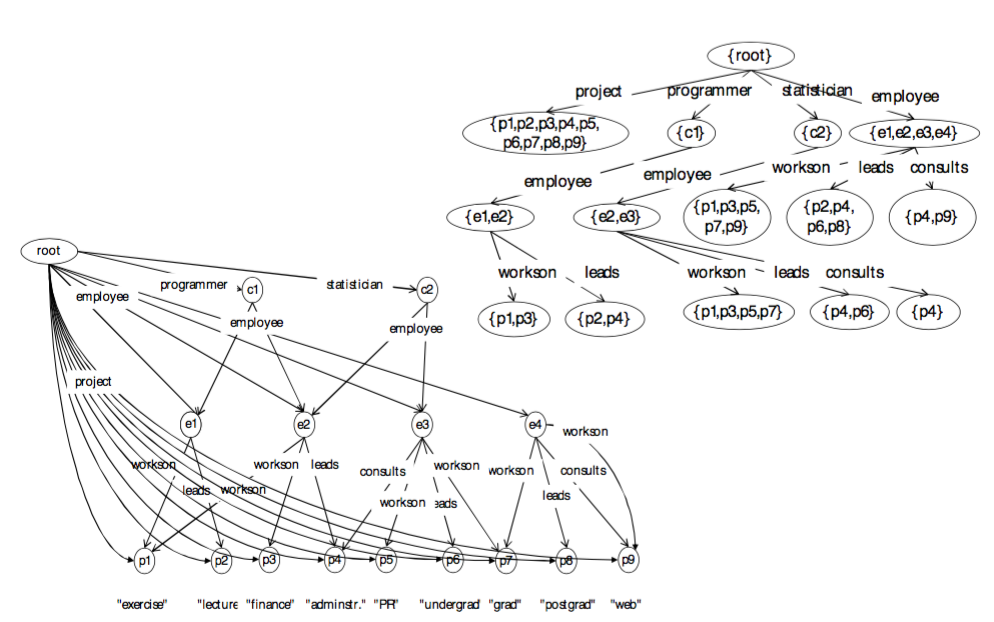
\includegraphics[width=\textwidth]{figures/data_guide.png}
\subsection{Schema Mapping}




\section{Social Graph}

In social graph mining, we often want to extract significant communities of users.

\subsection{Community evaluation}

Before extracting communities from a social graph, we need to define what is a strong community (well defined) and what is a weak communities (weak bounds between members).

\subsubsection{Strong or weak community}

For a given vertex $i$ we define
\begin{itemize}
  \item the internal degree $k_i^{int}$ the number of edges from $i$ going to another vertex of the community
  \item the external degree $k_i^{ext}$ the number of edges from $i$ going to a vertex outside of the community
\end{itemize}

For a node $i$ correctly assigned to a community $C$, we should have a high $k_i^{int}$ and a low $k_i^{ext}$. More formally

\[
  \sum_{i\in C} k_i^{int}(C) > \sum_{i\in C} k_i^{out}(C)
\]

\subsubsection{Modularity}

Modularity measures how well a graph $G$ is partitioned into communities $S$

\paragraph{Modularity.}
  \[
    Q \propto \sum_{s \in S} (\text{\# edges within } s) - (expected \text{ \# edges within } s)
  \]
  The expected value is computed on a graph with same degree distribution but random connections (null model).


\paragraph{Normalized modularity.}
  \[
    Q(G,S) = \underbrace{\frac 1 {2m}}_{\text{normalize}} \sum_{s\in S, i,j\in s} \l(A_{ij} - \frac{k_ik_j}{2m}\r)
  \]
  and $-1<Q<1$


Modularity is positive if the intra connection exceeds the expected number. A partitioning is significant if $Q>0.3,0.7$. We can use modularity to know when to stop community extraction algorithm (pick).

\subsection{Community extraction}

% We build a similarity matrix ($A_{ij}$ how node $i$ and $j$ are similar) from the adjacency matrix.

Hierarchical clustering algorithms identifies groups of nodes with high similarity. We can distinguish two strategies:

\begin{itemize}
  \item \textbf{Agglomerative algorithm:} merge nodes and communities with high similarity
  \item \textbf{Divisive algorithm:} split communities by removing links connecting nodes with low similarity (smallest cut)
\end{itemize}

In both strategy, we need a stopping point for the iterative process. Either we chose an arbitrary number of communities $k$ or we use a criteria (see modularity).

\paragraph{Girvan-Newman method.} Divisive hierarchical clustering based on edge betweenness. Iteratively remove edge of highest betweenness. Runs in $O(ln^2)$, $O(n^3)$ for sparse graph.

\paragraph{Louvain Modularity.} Greedy optimization in $O(n\log n)$, find small communities locally and then group smallest communities as simple nodes.

\subsubsection{Edge betweenness}

\paragraph{Edge betweenness.}
  Number of shortest paths passing over an edge (max $n(n-1)$)


\paragraph{Random walk betweenness.}
  Given two nodes $i$ and $j$, $x_{ij}$ is the probability that the edge between $i$ and $j$ is taken by a walk averaged over all the random walks between the pairs of node of the graph.


\subsubsection{How to compute betweenness ?} 

Repeat for each node, but let take $A$ w.l.o.g. (see \cref{fig:betweenness})

\begin{itemize}
  \item BFS from node $A$, all nodes are layered
  \item For each node $i$, count the number of shortest paths arriving to $i$. Recursively sum up the count of the parents (assigning 1 to node $A$).
  \item Assign edge values bottom up, each node has value $1 + \sum ($child edges weight$)$, to distribute proportionally to its parents according to their weight
\end{itemize}


\begin{figure}
  \centering
  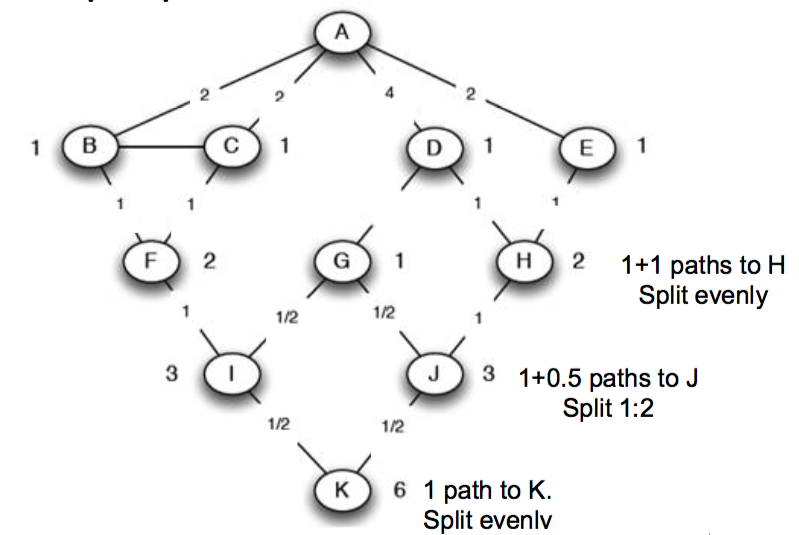
\includegraphics[width=1\linewidth]{figures/betweenness_computation.png}
  \caption{Betweenness computation - BFS, top down node weighting, bottom up edge values}
  \label{fig:betweenness}
\end{figure}

\subsection{Random graphs}

\paragraph{Small world graphs.}
  Graph for which most nodes are not neighbors of one another but most nodes can be reached from any other node by a small number of hops


\paragraph{Milgram's experiment.} Send a message from Nebraska to Massachusetts, from people to friends/relatives (mean of 5-6 hopes)

The experiment rises two problem, how to explain that there exists such short paths in  the social graph, and how to actually find these shortest paths efficiently ?

\subsubsection{Random graph model $G(n,p)$}

Simplest model, take $n$ nodes, connect each pair of nodes with probability $p$. It has the following properties

\begin{itemize}
  \item \textbf{low diameter}, expected distance between two nodes is $\log_k n$ with $k$ the average out degree,
  \item a pair $(i,j) \in V^2$ picked uniformly at random is connected by a short path with high probability
  \item \textbf{low clustering} coefficient (inaccurate for social graph modeling)
\end{itemize}

\paragraph{Diameter.}
  The diameter of a graph $G$ is the longest shortest path between any pair of nodes.

\paragraph{Local clustering coefficient.}
  The local clustering coefficient is the proportion of neighbors connected for a given node. Formally for a given edge $i$ with neighbors $N$ and edges between them $E$
  \[
    C_i = \frac { 2|E|}{|N|(|N|-1)}
  \]

\paragraph{Global clustering coefficient.}
  Average of the local clustering coefficient.
  \[
    C = \frac 1 n \sum_i^n C_i
  \]

\subsubsection{Watts and Strogatz model}

Random rewiring of regular graph: take a recular graph and with probability $p$ rewire each link to a randomly selected node. Resulting graph has properties, both of regular and random graphs, see \cref{fig:watts_strogatz}.

\begin{figure}
  \centering
  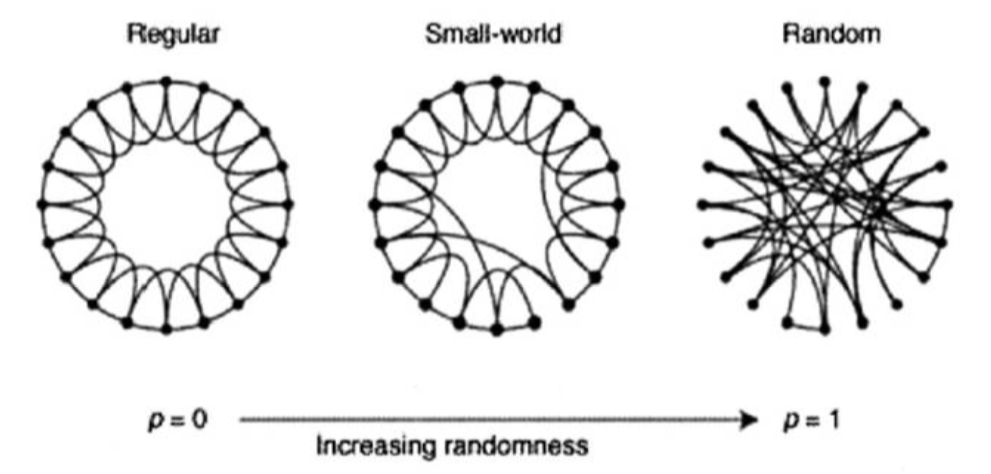
\includegraphics[width=1\linewidth]{figures/watts_strogatz_graph.png}
  \caption{Watts Strogatz rewiring construction}
  \label{fig:watts_strogatz}
\end{figure}

\subsubsection{Efficient search algorithm (Kleinberg’s model)}

\begin{itemize}
  \item Embed a graph into an $d$-dimensional grid to define a distance function ($l-2$ norm for instance)
  \item each node is connected to $p$ of its closest neighbor (short range links) + $q$ random nodes (long range links) according to a distribution
  \[
    \P{u \leftrightarrow v} \propto \text{dist}(u,v)^{-r}
  \]
\end{itemize}

Decentralized routing algorithm performs well if and only if $r=$ dimension of the space. If $r$ is too small, we go far but struggle to converge, if $r$ is too high we stay among our neighbors, hard to reach the neighborhood of the target.

For $r=0$ we chose the long range links uniformly, like a random graph. there exist short paths between every pair of vertex but there is no decentralized algorithm capable finding these paths efficiently.

\paragraph{Routing cost.} With $O(1)$ long range link $O(\log^2 n)$, and with $O(\log n)$ long range links $O(\log n)$.


\end{document}
